\documentclass[a4paper,12pt]{article}
\usepackage{graphicx}
\usepackage{float}
\usepackage{titling}

\setlength{\droptitle}{-14em}
\title{Temperature Autocorrelation Analysis}
\author{Zhongbin Hu}
\date{\today}

\begin{document}

\maketitle
\section{Results}

\subsection{Correlation Coefficient Calculation}
  \begin{figure}[ht]
    \centering
    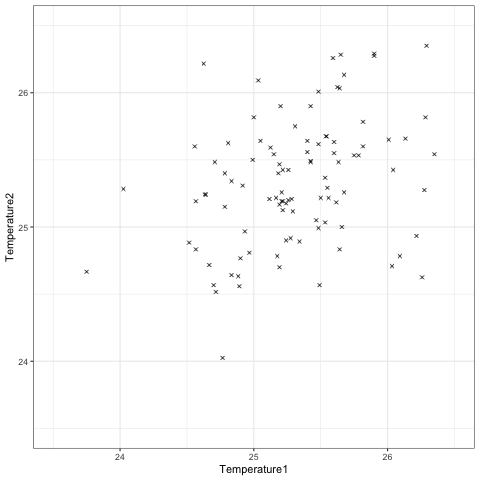
\includegraphics[width=0.7\textwidth]{../data/ats_plot.png}
    \caption{Temperature between consecutive years}
  \end{figure}
  In the analysis of consecutive yearly temperatures, the correlation coefficient is found to be 0.3261697. This value suggests a moderate, albeit not strong, linear relationship between temperatures of one year and the next. The graphical representation of this data also supports the observation of a weak correlation in year-to-year temperature variations.

\subsection{Random Time Series Multiple Calculations}
  \begin{figure}[ht]
    \centering
    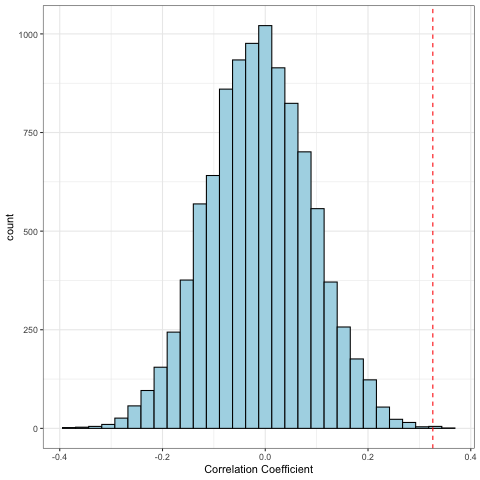
\includegraphics[width=0.7\textwidth]{../data/ats_random_plot.png}
    \caption{Statistical distribution and count of correlation coefficients.}
  \end{figure}
  By conducting $10,000$ random permutations, the graph clearly shows that most of the test correlation coefficients cluster near zero. The red dashed line on the graph signifies the correlation coefficient calculated from the original data, without random permutations. Notably, almost all the correlation coefficients obtained from the tests exceed the original one. This suggests a presence of correlation between the initial temperature data and the time series.
\end{document}
